\chapter{子空间、投影算符与作为纠缠的测量}

贝尔定理留下了两个悬而未决的问题。当一对粒子中的一个受到扰动、被吸收或被测量时，纠缠还剩下什么？而究竟是什么，把一次普通的相互作用变成了一次测量？通往答案的路径要经过初等线性代数。性质是子空间，概率是投影算符的期望值，而测量仪器则是另一个量子系统，对象与之发生纠缠。

\section{开篇动机：纠缠、定域性与测量}

假设一个单态已被分离到两个相距遥远的部分，并且其中一部分被测量。量子场论是否必须描述它们之间的某种虚交换？在远侧不会发生任何可探测的事件，也不会有可用的信息到达那里。人们可以用磁场在局部旋转其中一个自旋，从而改变联合态的具体形式，而纠缠量在该局部操作下保持不变。纠缠的定量度量将在后面讨论；眼下要点在于，两个不再相互作用的系统，不可能仅仅通过局限于一侧的操作来改变它们共享的纠缠。

\begin{classroomqa}
\lecturetimestamp{00:00:22}
\audiencequestion{对类空间隔的单态中的一个成员进行测量，是否需要与另一个成员发生某种虚交换？}
\lecturerresponse{在另一侧不会发生任何可探测的交换。局部操作可以旋转其中一个因子，并改变联合态被写出的形式，但它本身不能发送信息，也不能改变跨越这一间隔所共享的纠缠。}
\end{classroomqa}

这就迫使我们对什么算作伙伴采取一种更宽泛的概念。如果纠缠对中的一个成员落入黑洞，另一个并不会不再纠缠；它会与黑洞的自由度发生纠缠，并且在蒸发之后，与发射出的辐射发生纠缠。同样的想法并不需要黑洞。把纠缠对中的一个成员丢进浴缸，让它与水剧烈混合。它的个体身份可能在多体态中丢失，但远处的粒子仍然与整个浴缸纠缠，并最终与逸出的水蒸气纠缠。

这不仅仅是一个关于持续性的故事。它也是一个关于可逆性的故事。如果相互作用能够产生纠缠，那么相互作用原则上也能够解除纠缠。解纠缠是可能的，但只有当这些系统重新接触并再次相互作用时才行。任何能以一种方式发生的事情，也能以另一种方式发生。

\begin{classroomqa}
\lecturetimestamp{00:04:45}
\audiencequestion{如果对纠缠对的两个自旋都进行测量，电子还会保持纠缠吗？一次测量就已经能使它们解纠缠吗？}
\lecturerresponse{测量可以消除它们之间的相互纠缠，而且一次测量就可能足够。要看清这一陈述意味着什么，而不是仅仅断言坍缩，我们必须把观察描述为系统与记录仪器之间的一种相互作用。}
\end{classroomqa}

这个问题设定了目标：把观察、波包的坍缩和纠缠联系起来。然而，在接近它之前，我们需要对子空间和投影算符有一个更清晰的说明，所用工具不超出论证所需。

\section{维数、线性相关与正交归一基}

因此，我们暂时停留在配备左矢、右矢和内积的有限维向量空间上。萨斯坎德尽可能从最基础的地方开始。他并不通过数列向量中的分量来定义维数。他抽象地定义它：向量空间的维数是在其中所能找到的线性无关向量的最大数目。

因此，一个集合 \(\{|v_i\rangle\}\) 是线性无关的，当关系式
\begin{equation}
\sum_i c_i |v_i\rangle = 0
\end{equation}
迫使所有系数 \(c_i\) 都为零时。等价地说，其中任何一个向量都不能写成其余向量的线性组合。

这里至关重要的是，正交性与无关性并不是同一回事。在三维中，人们可以有三个完全不正交的向量，而它们却是线性无关的。关键在于其中一个能否由另外两个构造出来。另一方面，在一个二维平面中，该平面内的任何第三个向量都必定线性相关于前两个。

\begin{figure}[htbp]
\centering
\includegraphics[width=0.56\textwidth]{lecture_06_figure_02.png}
\caption{黑板上画出的三个向量。讲座用这幅草图把正交性的概念与线性无关性的概念区分开来，然后强调在平面中第三个向量相关于前两个。}
\lectureframe{00:09:35}
\end{figure}

\begin{figure}[htbp]
\centering
\begin{tikzpicture}[scale=1.2]
\draw[->] (0,0) -- (2.3,0);
\draw[->] (0,0) -- (2.0,2.0);
\draw[->] (0.35,0.95) -- (1.05,1.45);
\fill (0,0) circle (1.2pt);
\end{tikzpicture}
\caption{黑板草图的极简重构。精确的系数关系并不能仅由该框架确定；其几何要点在于，在二维平面中第三个向量并不独立。}
\end{figure}

这正是该草图的关键。若空间是二维的，则线性无关向量的最大数目为二。若空间是三维的，则为三。更一般地，若空间的维数为\(d\)，则在给定内积的情况下，可以找到\(d\)个相互正交的单位向量张成该空间。这些就是基向量。Susskind明确表示他在这里不会证明该定理。他只想要结论：一旦这样的基存在，空间中的每个向量都可以用它展开。

\begin{classroomqa}
\lecturetimestamp{00:10:58}
\audiencequestion{空间自由度的数目与态空间的维数相同吗？}
\lecturerresponse{不相同。在房间中运动的粒子有三个空间坐标，却拥有数量极其庞大的相互正交的量子态。位形空间的维数与希尔伯特空间的维数是不同的概念；使用有限维的例子只是为了清晰地揭示其中的逻辑。}
\end{classroomqa}

\section{基展开、并矢与恒等式的分解}

现在选取一组正交归一基\(\{|n\rangle\}\)，其中\(n=1,\dots,d\)。此时黑板上的内容尤为清晰而紧凑：

\begin{figure}[htbp]
\centering
\includegraphics[width=0.62\textwidth]{lecture_06_figure_03.png}
\caption{正交归一基与任意态的展开。}
\lectureframe{00:14:15}
\end{figure}

我们写出
\begin{align}
\langle m|n\rangle &= \delta_{mn}, \\
|\psi\rangle &= \sum_n a_n |n\rangle.
\end{align}
这里\(\delta_{mn}\)是克罗内克{\proseunicodefont δ}：当\(m=n\)时它为\(1\)，否则为\(0\)。

\paragraph{推导实例。}系数通过向基上投影而恢复。左乘\(\langle m|\)：
\begin{align}
\langle m|\psi\rangle
  &= \sum_n a_n \langle m|n\rangle \\
  &= \sum_n a_n \delta_{mn} \\
  &= a_m.
\end{align}
因此系数就是
\begin{equation}
a_m = \langle m|\psi\rangle.
\end{equation}
该系数是一个普通的复数，因此可以放在右矢的任意一侧而不改变任何东西。

若将系数代回展开式，我们得到
\begin{equation}
|\psi\rangle = \sum_n |n\rangle \langle n|\psi\rangle.
\end{equation}
这表明对象\(|n\rangle\langle n|\)，更一般地\(|a\rangle\langle b|\)，应当被理解为算符。这正是下一步。并矢的作用为
\begin{equation}
\bigl(|a\rangle\langle b|\bigr)|\psi\rangle = \langle b|\psi\rangle\,|a\rangle.
\end{equation}
左矢提取出一个复数；右矢提供所得到的方向。这就是Susskind从向量通向算符的低技术路线。

现在以算符的方式重新解读先前的展开。由于对每个\(|\psi\rangle\)都有
\begin{equation}
|\psi\rangle = \left(\sum_n |n\rangle\langle n|\right)|\psi\rangle
\end{equation}
括号中的算符必定是恒等算符：
\begin{equation}
\sum_n |n\rangle\langle n| = I.
\end{equation}
这就是恒等式的分解。

\begin{figure}[htbp]
\centering
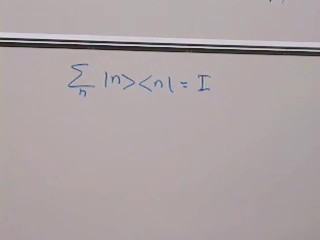
\includegraphics[width=0.60\textwidth]{lecture_06_figure_07.png}
\caption{完成后的黑板上的恒等式分解。}
\lectureframe{00:18:30}
\end{figure}

\begin{classroomqa}
\lecturetimestamp{00:18:39}
\audiencequestion{恒等式分解中的向量必须是基吗？}
\lecturerresponse{是的。该推导同时用到了归一化和相互正交性，并且求和必须遍历一组完备基。任意一组向量并不能分解恒等式。}
\end{classroomqa}

恒等算符本身就是向整个空间的投影算符。每个向量都是\(I\)的本征向量，且每个本征值都是\(+1\)。

\begin{classroomqa}
\lecturetimestamp{00:19:14}
\audiencequestion{恒等式分解是否意味着每个向量都具有本征值一？}
\lecturerresponse{是的，对于恒等算符而言。它的特殊之处在于每个向量都是它的本征向量，且对每个态都有\(I|\psi\rangle=|\psi\rangle\)。}
\end{classroomqa}

\section{作为子空间的性质与投影算符}

有了这套工具，讲座给出了其核心的概念性修正。诸如\(k=\lambda\)这样的性质一般并不是一个向量。它是一个完整的子空间。

设\(k\)是一个厄米可观测量，并假设
\begin{equation}
k|A\rangle = \lambda |A\rangle, \qquad
k|B\rangle = \lambda |B\rangle,
\end{equation}
其中\(|A\rangle\)与\(|B\rangle\)线性无关。那么任意线性组合都具有相同的本征值：
\begin{align}
k\bigl(\alpha|A\rangle+\beta|B\rangle\bigr)
  &= \alpha k|A\rangle + \beta k|B\rangle \\
  &= \alpha \lambda |A\rangle + \beta \lambda |B\rangle \\
  &= \lambda\bigl(\alpha|A\rangle+\beta|B\rangle\bigr).
\end{align}
因此\(\lambda\)的本征空间对加法和数乘封闭。它是一个向量子空间。

讲座的第一个具体例子是一个双自旋系统。态
\begin{equation}
|ud\rangle,\qquad |uu\rangle
\end{equation}
具有不同的第二个自旋值，但第一个自旋值相同：在两种情况下第一个自旋都朝上。因此它们张成了第一个自旋满足\(\sigma_3=+1\)的子空间。

\begin{figure}[htbp]
\centering
\includegraphics[width=0.46\textwidth]{lecture_06_figure_04.png}
\caption{两个第一个自旋朝上的双自旋态。}
\lectureframe{00:23:27}
\end{figure}

这一点值得保留：一个性质不一定是一个态。它是具有相同本征值的整整一组态。

为了避免黑板上短暂出现的记号混淆，我们将用大写字母\(A,B,\dots\)表示特定的本征向量，并用小写\(a,b,\dots\)作为求和指标，遍历本征子空间的一组正交归一基。如果\(\{|a\rangle\}\)是子空间\(k=\lambda\)的一组这样的基，那么到该子空间的投影算符为
\begin{equation}
\Pi_{k=\lambda}=\sum_a |a\rangle\langle a|.
\end{equation}
这不过是限制在该子空间上的恒等算符。如果\(|\psi\rangle\)已经位于该子空间中，投影算符将其原样返回。如果\(|\psi\rangle\)有一部分位于其外，投影算符丢弃正交的剩余部分，只保留位于子空间内的分量。

\section{概率公设、相容性质与贝尔回顾}

一旦性质被重新解释为子空间，概率公设就呈现出最简洁的形式。如果\(|\psi\rangle\)是归一化的，那么它具有性质\(k=\lambda\)的概率为
\begin{equation}
P(k=\lambda)=\langle\psi|\Pi_{k=\lambda}|\psi\rangle.
\end{equation}

\begin{figure}[htbp]
\centering
\includegraphics[width=0.58\textwidth]{lecture_06_figure_05.png}
\caption{到\(k=\lambda\)本征子空间的投影算符。黑板上的布局已经为下一步做好了准备：将投影算符夹在\(\langle\psi|\)与\(|\psi\rangle\)之间。}
\lectureframe{00:31:09}
\end{figure}

代入投影算符的并矢形式：
\begin{align}
P(k=\lambda)
  &= \left\langle \psi \left| \sum_a |a\rangle\langle a| \right| \psi \right\rangle \\
  &= \sum_a \langle\psi|a\rangle\langle a|\psi\rangle \\
  &= \sum_a |\langle a|\psi\rangle|^2.
\end{align}
这正是讲座中的解释：该性质的总概率等于该性质能够出现的所有正交方式的概率之和。

对于双自旋系统中第一个自旋朝上的情形，相关子空间由\(|uu\rangle\)和\(|ud\rangle\)张成，因此
\begin{equation}
\Pi_{\sigma_3=+1}=|uu\rangle\langle uu|+|ud\rangle\langle ud|.
\end{equation}
在讲座的简写中，这也被写作
\begin{equation}
\Pi_{\sigma_3=+1}=\frac{1+\sigma_3}{2},
\end{equation}
其中第二个自旋上的恒等算符被省略了。

\begin{classroomqa}
\lecturetimestamp{00:33:04}
\audiencequestion{可观测量、性质和投影算符之间有什么区别？}
\lecturerresponse{可观测量是厄米算符\(k\)。性质\(k=\lambda\)由其本征子空间表示，意味着测量\(k\)必定会得到\(\lambda\)。投影算符\(\Pi_{k=\lambda}\)分离出该子空间，其期望值给出该性质存在的概率。}
\end{classroomqa}

\begin{classroomqa}
\lecturetimestamp{00:34:07}
\audiencequestion{简并本征向量\(A\)和\(B\)是否必须已经正交，它们是否是整个空间的基？}
\lecturerresponse{原始本征向量不必正交，但总可以在它们的本征子空间内选取一组正交归一基。它只是该子空间的基；要张成整个空间还需要额外的正交方向。投影到每个子空间基向量上再相加，就得到到该子空间的投影。}
\end{classroomqa}

\begin{classroomqa}
\lecturetimestamp{00:35:33}
\audiencequestion{在\(k|A\rangle=\lambda|A\rangle\)中，符号\(a\)与投影算符中求和的\(a\)含义相同吗？}
\lecturerresponse{不相同。前者表示一个特定的本征向量，而求和号下的指标遍历本征子空间的一组正交归一基中的每一个向量。使用不同的记号可以防止将固定的标签误认为哑求和指标。}
\end{classroomqa}

\begin{classroomqa}
\lecturetimestamp{00:37:15}
\audiencequestion{投影算符公式中的内积是概率还是概率幅？}
\lecturerresponse{每个\(\langle a|\psi\rangle\)是一个概率幅。乘以它的复共轭得到概率，将这些概率对实现\(k=\lambda\)的所有正交方式求和，就得到该性质的总概率。}
\end{classroomqa}

讲座接着问如何组合性质。假设我们有两个相容的性质，由对易的投影算符\(P_k\)和\(P_\ell\)表示。用讲座中的语言，AND陈述由乘积表示：
\begin{equation}
\Pi_{k=\lambda\,\wedge\,\ell=\mu}=P_kP_\ell=P_\ell P_k.
\end{equation}
逻辑很简单。\(P_k|\psi\rangle\)位于\(k=\lambda\)子空间中。因为算符对易，\(P_\ell P_k|\psi\rangle=P_kP_\ell|\psi\rangle\)，所以同一个向量也位于\(\ell=\mu\)子空间中。因此乘积投影到同时成立的性质上。相应的概率为
\begin{equation}
P(k=\lambda,\ell=\mu)=\langle\psi|P_kP_\ell|\psi\rangle.
\end{equation}

该论证的第一步值得单独展示。对于任意态，
\begin{equation}
k\bigl(P_k|\psi\rangle\bigr)=\lambda P_k|\psi\rangle,
\end{equation}
所以\(P_k|\psi\rangle\)位于\(k=\lambda\)本征子空间中。如果\(P_k\)和\(P_\ell\)对易，乘积可以写成任一投影算符在左的形式，因此同时属于两个子空间。

\begin{figure}[htbp]
\centering
\includegraphics[width=0.44\textwidth]{lecture_06_figure_06.png}
\caption{投影后的态作为本征子空间中的向量。}
\lectureframe{00:41:57}
\end{figure}

\begin{figure}[htbp]
\centering
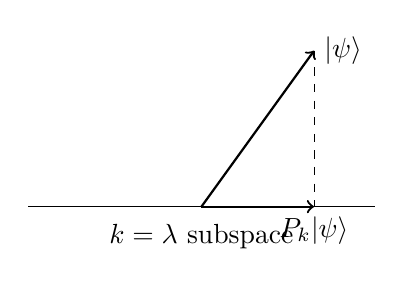
\begin{tikzpicture}[scale=1.1]
\draw (-2,0) -- (2,0);
\draw[->,thick] (0,0) -- (1.3,1.8) node[right] {$|\psi\rangle$};
\draw[dashed] (1.3,1.8) -- (1.3,0);
\draw[->,thick] (0,0) -- (1.3,0) node[below] {$P_k|\psi\rangle$};
\node at (0,-0.35) {$k=\lambda$ subspace};
\end{tikzpicture}
\caption{将任意向量投影到\(k=\lambda\)本征子空间中。}
\end{figure}

\begin{figure}[htbp]
\centering
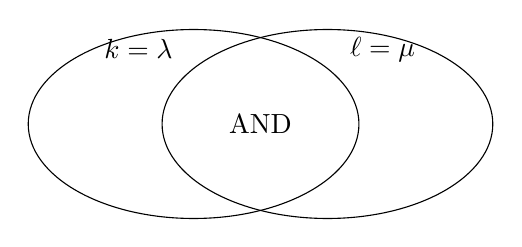
\begin{tikzpicture}[scale=1.0]
\draw (0,0) ellipse (2.1 and 1.2);
\draw (1.7,0) ellipse (2.1 and 1.2);
\node at (-0.7,0.95) {$k=\lambda$};
\node at (2.4,0.95) {$\ell=\mu$};
\node at (0.85,0) {AND};
\end{tikzpicture}
\caption{对易投影算符的AND陈述背后相交子空间图像的重构。}
\end{figure}

\begin{figure}[htbp]
\centering
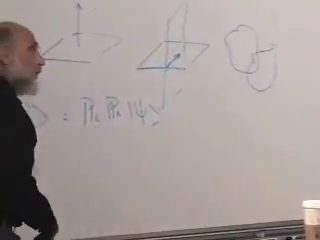
\includegraphics[width=0.66\textwidth]{lecture_06_figure_08.png}
\caption{黑板上关于对易投影算符选出同时本征子空间的论证。}
\lectureframe{00:45:20}
\end{figure}

\begin{classroomqa}
\lecturetimestamp{00:44:42}
\audiencequestion{同时具有的性质与经典逻辑中的交是同一回事吗？}
\lecturerresponse{是的。对于对易投影算符，\(P_kP_\ell\)投影到两个本征子空间的交上。若该交只包含零向量，则没有任何非零态同时具有这两个性质。}
\end{classroomqa}

为完整起见，相容的“或”子空间上的投影算符为
\begin{equation}
P_{k\lor\ell}=P_k+P_\ell-P_kP_\ell .
\end{equation}
当各备选互斥时，\(P_kP_\ell=0\)，此式化为求和\(P_k+P_\ell\)。只要两个子空间有重叠，这一减法就必不可少，因为它们的交不能被重复计入。

于是相容性本身又被联系回物理实例。在一个双自旋系统中，第一个自旋的任意分量\(\sigma_i\)与第二个自旋的任意分量\(\tau_j\)对易：
\begin{equation}
[\sigma_i,\tau_j]=0.
\end{equation}
相反，同一自旋的不同分量并不对易：
\begin{equation}
[\sigma_1,\sigma_3]\neq 0.
\end{equation}
这就是为什么可以测量两个分离自旋各自的一个分量，却不能同时测量同一自旋的两个不同分量。

\begin{classroomqa}
\lecturetimestamp{00:46:12}
\audiencequestion{相容可观测量有哪些具体例子？}
\lecturerresponse{作用于第一个自旋的任意算符与作用于第二个自旋的任意算符对易，因为它们作用在不同的张量因子上。位置分量\(x,y,z\)是另一族相容量。相反，同一自旋的两个不同分量，或者位置与其共轭动量，并不对易。}
\end{classroomqa}

\begin{classroomqa}
\lecturetimestamp{00:47:26}
\audiencequestion{子系统是否必须指不同的粒子？}
\lecturerresponse{不是。它指的是一组被独立指定的自由度。不同粒子给出最简单的张量因子，但当算符结构允许时，同一个粒子的不同自由度也可以被分开处理。}
\end{classroomqa}

\begin{classroomqa}
\lecturetimestamp{00:48:37}
\audiencequestion{既然不同子系统上的这么多算符都对易，那么一个简单的不相容对是什么？}
\lecturerresponse{同一自旋的两个分量给出了标准例子：\(\sigma_1\)与\(\sigma_3\)不对易，因此没有任何仪器能同时赋予二者确定值。非零的矩阵对易子就是代数上的判据。}
\end{classroomqa}

现在 Susskind 重新审视 Bell 定理。他并不重做上一讲的算术。他用新的语言重建其逻辑。经典不等式以概率形式写为
\begin{equation}
P(A\wedge \neg B)+P(B\wedge \neg C)\ge P(A\wedge \neg C).
\end{equation}
这是经典集合逻辑的定理，而非量子力学的定理。在单态中，自旋沿任意共同轴反向排列，因此关于第一个自旋的“非”陈述可以换成关于第二个自旋的相应肯定陈述。这就使人能够把该不等式改写为关于双自旋系统联合性质的陈述。

略去未触及因子上的恒等算符后，讲座中出现的单性质投影算符为
\begin{equation}
\frac{1+\sigma_3}{2},\qquad
\frac{1+\frac{\tau_1+\tau_3}{\sqrt2}}{2},\qquad
\frac{1+\frac{\sigma_1+\sigma_3}{\sqrt2}}{2},\qquad
\frac{1+\tau_1}{2}.
\end{equation}
因此三个相关的联合投影算符为
\begin{align}
\Pi_1 &= \frac{1+\sigma_3}{2}\,\frac{1+\frac{\tau_1+\tau_3}{\sqrt2}}{2}, \\
\Pi_2 &= \frac{1+\frac{\sigma_1+\sigma_3}{\sqrt2}}{2}\,\frac{1+\tau_1}{2}, \\
\Pi_3 &= \frac{1+\sigma_3}{2}\,\frac{1+\tau_1}{2}.
\end{align}

\begin{figure}[htbp]
\centering
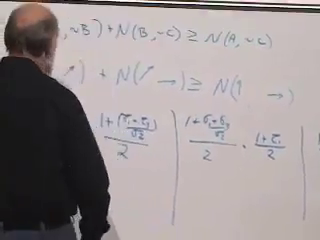
\includegraphics[width=0.68\textwidth]{lecture_06_figure_09.png}
\caption{三种分析器选择写成单自旋投影算符的乘积。}
\lectureframe{01:01:45}
\end{figure}

讲座以熟悉的未归一化黑板形式谈到单态
\begin{equation}
|\Psi_{\mathrm{singlet}}\rangle \propto |ud\rangle-|du\rangle.
\end{equation}
这里比例符号已经足够。对逻辑而言重要的是态本身，尤其是相对符号，而不是整体归一化。在单态中计算\(\langle \Pi_1\rangle+\langle \Pi_2\rangle\)相对于\(\langle \Pi_3\rangle\)，得到上一讲所获得的违背。重要的结论正是 Susskind 口头强调的那一个：量子力学并不是伪装的经典集合论。

\begin{classroomqa}
\lecturetimestamp{00:52:31}
\audiencequestion{如果自旋向上和自旋向下正交，那么负号是否意味着一个 ket 是另一个的负？}
\lecturerresponse{不是。\(|u\rangle\)与\(|d\rangle\)是不同的正交向量。相对符号属于诸如\(|ud\rangle-|du\rangle\)这样的叠加态，并能改变其物理性质；只有乘在整个态上的整体符号才无关紧要。}
\end{classroomqa}

\begin{classroomqa}
\lecturetimestamp{00:53:06}
\audiencequestion{Bell 不等式是否对每个量子态和每一种性质选择都被违背？}
\lecturerresponse{不是。许多态和许多轴的选择都满足某个特定的 Bell 不等式。违背与否取决于态和所选可观测量二者。改变中间角和最终角会改变这一检验是否暴露出非经典关联。}
\end{classroomqa}

\begin{classroomqa}
\lecturetimestamp{01:02:47}
\audiencequestion{当某个特定态违反、或恰好满足这个贝尔不等式时，可以得出什么结论？}
\lecturerresponse{违反证明了所观测到的统计不可能来自推导中所用的经典集合逻辑。满足某个选定的不等式本身并不能使该态成为经典的，因为选择另一组性质可能会揭示出违反。}
\end{classroomqa}

\section{贝尔之后的定域性}

投影算符的计算不仅仅是一种符号游戏。设想反复制备处于单态基态的相关联对，将两个成员分开，并把这样等同制备的系综分成三大组。第一组测量\(0^\circ\)和\(45^\circ\)设置，第二组测量\(45^\circ\)和\(90^\circ\)设置，第三组测量\(0^\circ\)和\(90^\circ\)设置。三组中的频率估计出不等式中的三个概率。

\begin{classroomqa}
\lecturetimestamp{01:04:30}
\audiencequestion{这三个贝尔概率实际上描述的是什么样的实验室安排？}
\lecturerresponse{一个源产生许多等同制备的纠缠对，并把两个成员发送到分离的分析器。把这些对分成三个系综，并对每个系综使用相应的一对分析器方向。对联合结果进行计数即可估计每个概率。带电粒子与反粒子可以通过场来分离；实际的贝尔检验则常常改用光子。}
\end{classroomqa}

\begin{classroomqa}
\lecturetimestamp{01:08:00}
\audiencequestion{经典集合证明只用了一个总体。三个分别测量的系综如何能检验它？}
\lecturerresponse{这个不等式既是关于计数的陈述，也是关于概率的陈述。如果三个样本都取自同一制备程序，那么它们的相对频率就估计出同一个共同系综的三个概率分布。等同制备是不可或缺的假设。}
\end{classroomqa}

那段贝尔回顾直接引出了仍然笼罩在房间里的那种物理上的不安。如果这些关联是真实的，为什么不能用它们来发送信号？

\begin{classroomqa}
\lecturetimestamp{01:09:41}
\audiencequestion{为什么不能用纠缠关联来发送超光速信息？}
\lecturerresponse{每一翼单独来看仍然只看到一段不可控制的随机序列。只有当两份记录通过普通的经典信道进行比较时，关联才会显现出来。然而，一个决定性的贝尔检验会安排选择和探测，使得任何光信号都无法及时在两翼之间通过，从而排除一种产生联合统计的定域通信机制。}
\end{classroomqa}

如果有足够的时间让光信号在装置之间传播，那么关联本身并不与相对论矛盾；人们可能只是发现了一种未被注意到的普通影响。那个尖锐的实验堵死了这条退路。用贝尔的话说，一个能重现这些关联的隐变量描述必须是非定域的，但非定域依赖并不等同于可控制的超光速信息。

\begin{classroomqa}
\lecturetimestamp{01:12:18}
\audiencequestion{角动量守恒对这个论证是本质性的吗？}
\lecturerresponse{不是。自旋只是一个方便的二态模型，并不是神圣不可缺的要素。任何具有所需纠缠态和备选测量基的二能级系统对，都可以展现出同样的逻辑结构。}
\end{classroomqa}

这段讨论并没有结束讲座；它为下一次转折清理了地基。贝尔已经教会我们，量子力学不是经典逻辑，但下一个问题有所不同。从操作上和数学上看，测量是什么，它又如何进入干涉的故事？

\section{有限态双缝、干涉以及作为纠缠的测量}

讲座现在更换模型。Susskind转向双缝实验，但他立刻把它简化为一个有限态问题，这样就可以使用同样的向量空间技术，而不必引入连续波动力学的全部机器。他甚至实际上说，这仍然是双缝实验，只不过被剥离到一小组基态上。

有一个源态\(|0\rangle\)、两个缝态\(|1\rangle\)和\(|-1\rangle\)，以及一组屏态\(|n\rangle\)。这些\(|n\rangle\)是正交归一的，因为不同的屏位置是不同的组态。讲座在此明确选择不仔细追踪归一化。幺正性被推迟。在这个阶段重要的是线性性。

\begin{figure}[htbp]
\centering
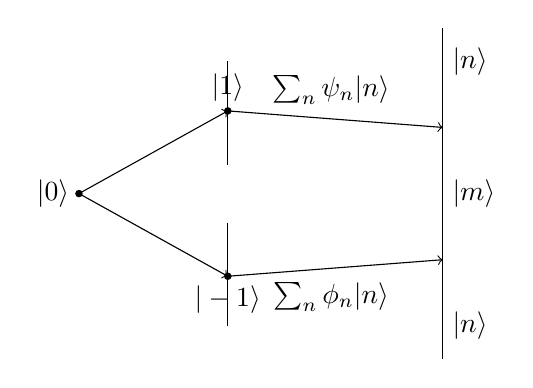
\begin{tikzpicture}[scale=1.05]
\fill (0,0) circle (1.3pt);
\node[left] at (0,0) {$|0\rangle$};

\draw (1.8,1.6) -- (1.8,0.35);
\draw (1.8,-0.35) -- (1.8,-1.6);
\fill (1.8,1) circle (1.3pt);
\fill (1.8,-1) circle (1.3pt);
\node[above] at (1.8,1) {$|1\rangle$};
\node[below] at (1.8,-1) {$|-1\rangle$};

\draw (4.4,2.0) -- (4.4,-2.0);
\node[right] at (4.4,1.6) {$|n\rangle$};
\node[right] at (4.4,0.0) {$|m\rangle$};
\node[right] at (4.4,-1.6) {$|n\rangle$};

\draw[->] (0,0) -- (1.8,1);
\draw[->] (0,0) -- (1.8,-1);
\draw[->] (1.8,1) -- (4.4,0.8);
\draw[->] (1.8,-1) -- (4.4,-0.8);

\node at (3.05,1.25) {$\sum_n \psi_n |n\rangle$};
\node at (3.05,-1.25) {$\sum_n \phi_n |n\rangle$};
\end{tikzpicture}
\caption{双缝实验的有限态版本：源态\(|0\rangle\)、两个缝态\(|1\rangle\)和\(|-1\rangle\)，以及屏基\(|n\rangle\)。}
\end{figure}

\begin{figure}[htbp]
\centering
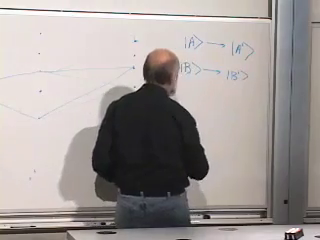
\includegraphics[width=0.68\textwidth]{lecture_06_figure_10.png}
\caption{线性演化规则\(A\to A'\)、\(B\to B'\)旁边的有限位置晶格。}
\lectureframe{01:18:00}
\end{figure}

由对称性，源演化为两个狭缝态的等振幅叠加：
\begin{equation}
|0\rangle \longrightarrow |1\rangle+|-1\rangle.
\end{equation}
现在让上狭缝态演化为
\begin{equation}
|1\rangle \longrightarrow \sum_n \psi_n |n\rangle,
\end{equation}
下狭缝态演化为
\begin{equation}
|-1\rangle \longrightarrow \sum_n \phi_n |n\rangle.
\end{equation}
这里的箭头表示时间演化，而不是同一时刻状态的相等。由线性性，
\begin{equation}
|1\rangle+|-1\rangle \longrightarrow \sum_n (\psi_n+\phi_n)|n\rangle.
\end{equation}
这就是关键规则。振幅在形成概率之前相加。

\begin{classroomqa}
\lecturetimestamp{01:21:59}
\audiencequestion{狭缝态\(|1\rangle\)如何能变成同样用整数\(n\)标记的态？这些右矢处于同一地点和同一时间吗？}
\lecturerresponse{这些标记指的是不同的时间切片。\(|1\rangle\)表示电子位于上狭缝，而右边的\(|n\rangle\)表示屏幕上可能的较晚位置。箭头表示时间演化，而不是同时位形之间的相等。}
\end{classroomqa}

\begin{classroomqa}
\lecturetimestamp{01:25:30}
\audiencequestion{这些振幅应当归一化吗？它们带有物理单位吗？}
\lecturerresponse{完整的演化必须保持总概率不变；这就是幺正性。这里省略了公共归一化因子，因为只有路径振幅的相加和相消才是重要的。当态被归一化时，任何标度因子都可以恢复。}
\end{classroomqa}

因此，到达屏幕位置\(m\)的概率为
\begin{align}
P_m &= |\psi_m+\phi_m|^2 \\
    &= |\psi_m|^2 + |\phi_m|^2 + \psi_m^*\phi_m + \phi_m^*\psi_m.
\end{align}
前两项是经典推理会得到的结果。后两项是干涉项。

\begin{figure}[htbp]
\centering
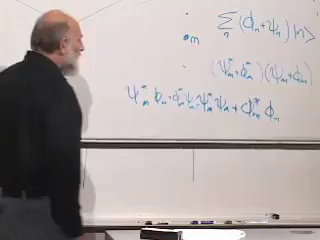
\includegraphics[width=0.68\textwidth]{lecture_06_figure_11.png}
\caption{黑板上的屏幕振幅及其四项概率展开。}
\lectureframe{01:29:20}
\end{figure}

在屏幕上的对称点，称之为\(m=0\)，对称性表明\(\psi_0=\phi_0\)。于是
\begin{equation}
P_0 = |\psi_0+\phi_0|^2 = |2\psi_0|^2 = 4|\psi_0|^2.
\end{equation}
在该点，双缝同时打开产生的概率是单缝概率的四倍，而不是两倍。这是相长干涉。

现在插入一个相移，使得\(\phi_0=-\psi_0\)。于是
\begin{equation}
P_0 = |\psi_0-\psi_0|^2 = 0.
\end{equation}
单独每个狭缝都允许到达该点，但把两者一起打开却可以使到达该点成为不可能。这是相消干涉。Susskind明确地详述了这有多么奇怪：在他看来，这和Bell一样奇异。

\begin{classroomqa}
\lecturetimestamp{01:33:14}
\audiencequestion{如果相移器或狭缝选择只在电子已经在飞行途中之后才改变，那会怎样？另一个狭缝需要时间来得知这件事吗？}
\lecturerresponse{答案取决于精确的时空安排，以及电子是否会遇到装置中被改变的部分。量子力学让态通过实际装置演化；概率仍然来自把适用的振幅相加。在能够评估定域性主张之前，必须精确地规定延迟选择方案。}
\end{classroomqa}

现在我们引入装置。有一个额外的二态系统，一个自旋，最初处于态\(|d\rangle\)。如果电子穿过上狭缝，它把该自旋翻转到\(|u\rangle\)。如果它穿过下狭缝，则使其保持不变。初始复合态是\(|0,d\rangle\)，而第一条更新规则变为
\begin{equation}
|0,d\rangle \longrightarrow |1,u\rangle + |-1,d\rangle.
\end{equation}
这一行就是讲座中测量的全部含义。电子的位置已经与装置中存储的记录纠缠在一起。

\begin{figure}[htbp]
\centering
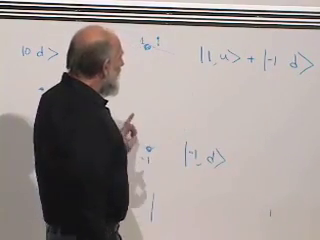
\includegraphics[width=0.66\textwidth]{lecture_06_figure_12.png}
\caption{探测器自旋把它的上和下记录与两个狭缝备选方案关联起来。}
\lectureframe{01:44:10}
\end{figure}

\begin{classroomqa}
\lecturetimestamp{01:40:20}
\audiencequestion{必须在两个狭缝处都放置探测器吗？}
\lecturerresponse{一个可靠的探测器就够了。如果它记录到穿过上狭缝，那么未改变的记录就标识出下狭缝这一备选方案，前提是每个透射电子都必须穿过两个开口之一。第二个探测器是可能的，但会增加另一个子系统，而不改变原理。}
\end{classroomqa}

\begin{classroomqa}
\lecturetimestamp{01:40:51}
\audiencequestion{为什么不说电子穿过两个狭缝？}
\lecturerresponse{没有路径记录时，态是相干叠加，不存在可回溯的路径事实。有了完整的哪条路径测量，装置在每次运行中记录这一个或那一个备选方案。在两个备选方案中持续存在的是态振幅，而不是两条分别被观测到的电子轨迹。}
\end{classroomqa}

\begin{figure}[htbp]
\centering
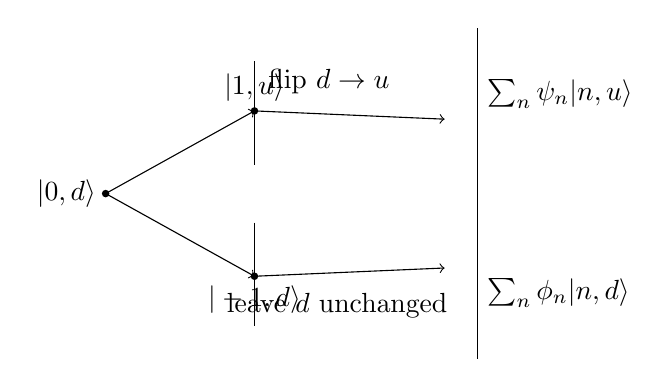
\begin{tikzpicture}[scale=1.05]
\fill (0,0) circle (1.3pt);
\node[left] at (0,0) {$|0,d\rangle$};

\draw (1.8,1.6) -- (1.8,0.35);
\draw (1.8,-0.35) -- (1.8,-1.6);
\fill (1.8,1) circle (1.3pt);
\fill (1.8,-1) circle (1.3pt);
\node[above] at (1.8,1) {$|1,u\rangle$};
\node[below] at (1.8,-1) {$|-1,d\rangle$};

\draw (4.5,2.0) -- (4.5,-2.0);
\node[right] at (4.5,1.2) {$\sum_n \psi_n |n,u\rangle$};
\node[right] at (4.5,-1.2) {$\sum_n \phi_n |n,d\rangle$};

\draw[->] (0,0) -- (1.8,1);
\draw[->] (0,0) -- (1.8,-1);
\draw[->] (1.8,1) -- (4.1,0.9);
\draw[->] (1.8,-1) -- (4.1,-0.9);

\node at (2.7,1.35) {flip \(d\to u\)};
\node at (2.8,-1.35) {leave \(d\) unchanged};
\end{tikzpicture}
\caption{测量作为与探测器自旋的纠缠。上路径翻转装置自旋；下路径使其保持不变。}
\end{figure}

假定如讲座所述，自旋在到达屏幕的途中不再发生任何进一步的变化。于是
\begin{align}
|1,u\rangle &\longrightarrow \sum_n \psi_n |n,u\rangle, \\
|-1,d\rangle &\longrightarrow \sum_n \phi_n |n,d\rangle.
\end{align}
因此，双缝均打开时的末态为
\begin{equation}
|\Psi_{\mathrm{final}}\rangle
  = \sum_n \psi_n |n,u\rangle + \sum_n \phi_n |n,d\rangle.
\end{equation}
这并不是单个电子自身各态的叠加，而是电子与仪器的纠缠态。

\begin{figure}[htbp]
\centering
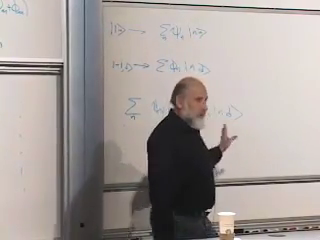
\includegraphics[width=0.68\textwidth]{lecture_06_figure_13.png}
\caption{两条路径的振幅到达屏幕时，携带着彼此正交的仪器记录。}
\lectureframe{01:47:35}
\end{figure}

计算到达位置 \(m\) 处概率的最简洁方法，是对电子子系统使用投影到该位置的投影算符：
\begin{equation}
\Pi_m = |m\rangle\langle m|\otimes I_{\mathrm{spin}}.
\end{equation}
将 \(\Pi_m\) 作用于末态，得到
\begin{equation}
\Pi_m |\Psi_{\mathrm{final}}\rangle
= |m\rangle\bigl(\psi_m|u\rangle+\phi_m|d\rangle\bigr).
\end{equation}
因此到达 \(m\) 的概率为
\begin{align}
P_m
  &= \langle \Psi_{\mathrm{final}}|\Pi_m|\Psi_{\mathrm{final}}\rangle \\
  &= \bigl(\psi_m^*\langle u|+\phi_m^*\langle d|\bigr)
     \bigl(\psi_m|u\rangle+\phi_m|d\rangle\bigr) \\
  &= |\psi_m|^2 + |\phi_m|^2
     + \psi_m^*\phi_m\langle u|d\rangle
     + \phi_m^*\psi_m\langle d|u\rangle.
\end{align}
但记录态彼此正交：
\begin{equation}
\langle u|d\rangle=0.
\end{equation}
所以交叉项消失：
\begin{equation}
P_m = |\psi_m|^2 + |\phi_m|^2.
\end{equation}
这就是讲座的数学要点。一旦路径信息被记录下来，干涉便消失，概率按经典方式相加。

\begin{classroomqa}
\lecturetimestamp{01:49:09}
\audiencequestion{叠加态 \(|1\rangle+|-1\rangle\) 与态 \(|1,u\rangle+|-1,d\rangle\) 之间有什么区别？}
\lecturerresponse{前者涉及一个系统处于两个位置的线性组合；不存在任何其他可与它纠缠的东西。后者涉及两个系统，并将路径与探测器自旋关联起来。读取自旋便可揭示关于路径的信息。}
\end{classroomqa}

\section{环境记录与部分测量}

有意建造的探测器并不是唯一的记录者。狭缝附近的原子、残余气体、热表面或任何其他自由度，都可能与路径发生关联。若其末态为 \(|E_1\rangle\) 和 \(|E_2\rangle\)，则路径态具有如下形式
\begin{equation}
|\Psi\rangle
=\sum_n\left(\psi_n|n\rangle|E_1\rangle
+\phi_n|n\rangle|E_2\rangle\right).
\end{equation}
此时干涉项被乘以重叠因子 \(\langle E_1|E_2\rangle\)。正交的记录使两条路径完全可区分，并彻底抹去干涉。完全相同的记录则使 \(\langle E_1|E_2\rangle=1\)，从而保留干涉。介于两者之间的重叠给出部分可见度。

\begin{figure}[htbp]
\centering
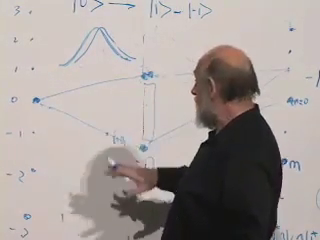
\includegraphics[width=0.68\textwidth]{lecture_06_figure_14.png}
\caption{重叠与分离的环境波包分别例示了部分路径记录与完全路径记录。}
\lectureframe{01:53:40}
\end{figure}

\begin{classroomqa}
\lecturetimestamp{01:50:48}
\audiencequestion{即使没有人有意去观测，狭缝附近的普通原子也会与经过的电子发生纠缠吗？}
\lecturerresponse{会。起作用的动词不是“知道”，而是物理关联。如果原子或周围气体受到足够扰动，使其后来的状态能够区分路径，那么它就记录了哪条路径的信息，并抑制了干涉。这正是此类实验需要隔离、低温，并且常常使用光子等弱相互作用粒子的原因。}
\end{classroomqa}

冷却使环境自由度接近其基态，从而减少偶然的记录。能隙也有帮助：如果入射粒子无法提供最低激发能量，环境就可能无法保留路径信息。反过来，带电粒子会通过其电场扰动附近物质，使电子干涉实验尤其苛刻。

\begin{classroomqa}
\lecturetimestamp{01:54:49}
\audiencequestion{真的能用单个电子获得干涉图样吗？}
\lecturerresponse{每个电子只造成一个局域化的击中。让粒子逐个通过，且间隔足够大，使它们无法相互作用，然后收集大量重复事件。累积的频率分布显示出干涉图样；单独一个事件只不过是一个小点。}
\end{classroomqa}

\begin{classroomqa}
\lecturetimestamp{01:55:59}
\audiencequestion{测量是破坏纠缠，还是产生纠缠？}
\lecturerresponse{哪条路径的相互作用在系统与仪器之间产生纠缠，而这种纠缠破坏了各备选之间的干涉。之后的测量可以使仪器与又一个系统关联，并可能对剩余态进行条件化，因此人们必须始终说明所讨论的是哪两个子系统以及哪一种干涉。}
\end{classroomqa}

\begin{classroomqa}
\lecturetimestamp{01:57:44}
\audiencequestion{能否减弱相互作用，使仪器只获得部分路径信息？}
\lecturerresponse{能。弱相互作用可能只以某个振幅使探测器翻转，留下非正交的记录态。于是两条路径仅部分可区分，干涉也仅部分减弱。测量越强，意味着可区分性越大，与记录的纠缠越强，而条纹可见度越低。}
\end{classroomqa}

因此，这里相关的坍缩是具体的：当路径信息已被沉积到另一个系统中时，它就是交叉项的丧失。没有记录时，振幅相加。当记录完全可区分时，它们的内积消失，概率相加。在这两个极端之间，测量强度和干涉可见度连续变化。